\begin{section}{Requisitos}
En este apartado se describe aquello que debe complir la infraestructura física para que los componentes de VMware Cloud Foundation funcionen de forma adecuada y que la configuración y mantenimiento de los componentes físicos sea simple a la hora de expandir el entorno.

% Teniendo en cuenta las capacidades físicas de la infraestructura, se ha elegido el modelo consolidado para el despliegue de VMware Cloud Foundation sobre la infraestructura.     La principal razón por las que se escoge este modelo es por el número de hosts ESXi.
% En los siguientes apartados se describen la arquitectura que se genera y la infraestructura requerida en cada capa.
%%%%%%%%%%%%%%%%%%%%%%%%%%%%%%%%%%%%%%
\begin{subsection}{Cómputo}
\begin{subsubsection}{Hosts ESXi}
    Para realizar el despliegue del primer WD (el Management Domain) se requieren al menos cuatro\footnote{Se reserva una cuarta parte de los recursos para que el \textit{management domain} permanezca activo en caso de caída de alguno de los hosts.} hosts ESXi con al menos un 128 GB de memoria RAM y un disco de arranque de 32 GB cada uno\footnote{Según la configuración establecida para el producto vSAN ReadyNode \cite{host-requirements}}. Para cada WD adicional solo se requiere un mínimo de tres hosts y la cantidad de memoria RAM depende de la finalidad del WD, por lo tanto para implementar el modelo de arquitectura estándar se requieren al menos siete hosts ESXi. Cada uno de los hosts debe tener al menos dos interfaces de red físicas (NIC) que soporten al menos 10 Gbit/seg de velocidad.
    
\end{subsubsection}
\end{subsection}
%%%%%%%%%%%%%%%%%%%%%%%%%%%%%%%%%%%%%%%
\begin{subsection}{Almacenamiento}
    En el Management Domain es obligatorio el uso de un \textit{datastore} de VMware vSAN, el cual necesita al menos tres hosts con recursos de almacenamiento para funcionar\footnote{VMware vSAN requiere un mínimo de tres hosts mientras que el Management Domain requiere un mínimo de cuatro hosts.}. Se debe aplicar la configuración All-Flash con discos SSD. Basándose en los perfiles que VMware establece para su producto vSAN Ready Node\cite{host-requirements}, cada host debe tener al menos un grupo de dos discos donde la cantidad de almacenamiento para la capa de capacidad debe ser de 4 TB y para la capa de caché de 200 GB. VMware vSAN soporta discos con adaptadores SAS, SATA o SCSI y estos pueden estar configurados en modo \textit{pass-through} o RAID 0. En cuanto a esto último, es preferible que los discos se configuren en modo \textit{pass-through} ya que permite que estos se puedan gestionar de forma independiente sin tener que apagar los hosts cuando es necesario retirar o añadir discos.
    Para WD adicionales se puede utilizar almacenamiento NFS en lugar de un \textit{datastore} de VMware vSAN, aunque la solución de VMware aporta mayor rendimiento y simplifica la administración de esta parte de la infraestructura física.
    % los discos de caché debe ser al menos un 10\% del tamaño total de los discos de capacidad,  y  \footnote{La capacidad de los discos descrita es la necesaria para desplegar el \textit{management domain} y un \textit{workload domain} adicional.}
\end{subsection}
%%%%%%%%%%%%%%%%%%%%%%%%%%%%%%%%%%%%%%%
\begin{subsection}{Red}
 \begin{subsubsection}{Switch Top Of Rack}
     Los hosts están colocados en racks, en un rack puede haber hosts pertenecientes a distintos WD. Para favorecer la alta disponibilidad y tolerancia a fallos de la infraestructura física, un rack debe tener dos switches Top Of Rack (TOR) y cada host debe tener una interfaz conectada a cada switch TOR, una capa superior de switches conecta los diferentes racks entre si. Todas las conexiones de la red física deben soportar \textit{Jumbo frames} (MTU hasta 9000 Bytes), etiquetado \textit{Quality of Service} (QoS) de tráfico y las VLAN configuradas para las redes del SDDC\footnote{Para el \textit{management domain} las subredes cuya VLAN debe ser configurada en la red física son la subred \textit{management}, la subred para VMware vSAN, la subred para overlay y la subred para VMware vSphere vMotion.}. Todos los switches TOR deben tener al menos dos interfaces 10 Gbit Ethernet como mínimo. 
 \end{subsubsection}
 \begin{subsubsection}{Servicios}
     En el SDDC se deben habilitar varios servicios requeridos por los componentes de VMware Cloud Foundation para su correcto funcionamiento.
     \begin{itemize}
         \item DNS: servidor de nombres para resolver todas las direcciones IP y \textit{hostnames} de los componentes del SDDC.
         \item DHCP: servidor para asignar de forma automática una dirección IP a los hosts que forman el SDDC.
         \item NTP: servidor de tiempo para sincronizar la hora de todos los componentes del SDDC.
         \item Router: se requiere para enrutar el tráfico que emiten todas las instancias del SDDC y para dar acceso a redes externas. Debe soportar enrutamiento dinámico BGP y debe tener configuradas las subredes y VLANS que se vayan a utilizar en la infraestructura.
         \item SMTP: servidor de correo utilizado por el componente VMware vRealize Automation.
         \item Active Directory: servidor de usuarios y grupos de usuarios que el SDDC utiliza como fuente para configurar el acceso a cada parte de la infraestructura virtual.
         \item Certificate Authority: se debe configurar una autoridad certificadora que genere certificados firmados para cada uno de los componentes de VMware Cloud Foundation. Permite establecer conexiones seguras cuando se accede a los componentes.
     \end{itemize}
 \end{subsubsection}
\end{subsection}


\end{section}
%%%%%%%%%%%%%%%%%%%%%%%%%%%%%%%%%%%%%%%
    %%%% DISEÑO ARQUI. FÍSICA %%%%%
% \begin{subsection}{Arquitectura e Infraestructura Físicas \cite{CFfisInfraestuctura}}
%     En este apartado se describen las principales características que tiene el entorno físico de un SDDC construído con VMware Cloud Foundation.


% \begin{subsubsection}{Red física}
% La topología de red en la capa física del SDDC de VMware Cloud Foundation se puede implementar mediante servicios de \underline{transporte} en la capa 2 o en la capa 3. El \underline{diseño en la capa 2} implica que la topología de la red incluya los dispositivos de capa 2 (\textit{Top of Rack Switches}) y los dispositivos de la capa 3 (routers, switches) [Fig. \ref{fig:transportlayer2}], por lo tanto las VLANs que se definan se deben implementar en la capa 2 y en la capa 3. Esto puede provocar problemas al aumentar el tamaño de la red ya que el número de VLANs disponible es más limitado, y problemas de compatibilidad ya que es posible que los dispositivos físicos tengan que ser del mismo proveedor. El \underline{diseño en la capa 3} implica que la topología de la red solo incluye a los dispositivos de capa 3 [Fig. \ref{fig:transportlayer3}]. Esto permite limitar la definición de VLANs a esa capa y el uso de enrutamiento dinámico con protocolos OSPF o BGP entre la capa 2 y 3. Así se consigue una mayor libertad a la hora de seleccionar los dispositivos físicos de red y que su configuración es más sencilla.
% \begin{figure}[h!]
%   \centering
%   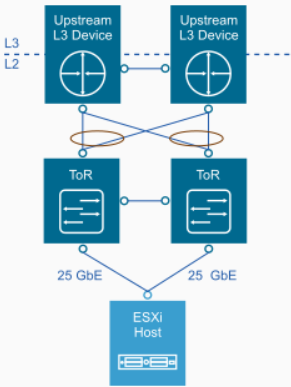
\includegraphics[width=0.3\textwidth]{imaxes/conceptosPrevios/transportlayer2.png}
%   \caption{Límite de las capas 2 y 3 cuando la topología se implementa con dispositivos de capa 2.}
%   \label{fig:transportlayer2}
% \end{figure}
% \FloatBarrier
% \begin{figure}[h!]
%   \centering
%   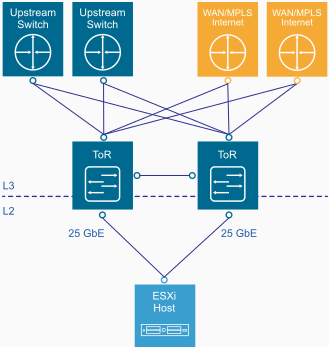
\includegraphics[width=0.3\textwidth]{imaxes/conceptosPrevios/transportNetLayer3.png}
%   \caption{Límite de las capas 2 y 3 cuando la topología se implementa con dispositivos de capa 3.}
%   \label{fig:transportlayer3}
% \end{figure}
% \FloatBarrier



% Como VMware Cloud Foundation abstrae la red física en una red virtual, la red física debe cumplir ciertos requisitos para que la red virtualizada sea robusta. Esta se debe mantener simple con configuraciones comunes en todos los switches, uso de VLANs y uso de enrutamiento dinámico, también debe ser escalable en cuanto a cantidad de hosts, ancho de banda y cantidad de rutas redundantes. Además, se debe tener en cuenta que cada tipo de tráfico tiene características diferentes, como por ejemplo el tráfico dedicado al almacenamiento a través de IP que suele usar mayor ancho de banda, por ello es necesario distinguir cada tipo de tráfico con protocolos \textit{Quality of Service} (QoS). El marcado de cada tipo de tráfico se realiza en el hipervisor ESXi a través de un vSphere Distributed Switch que soporta QoS tanto en la capa 2 como en la capa 3. En la capa 2 se utiliza  un campo de tres bits llamado \textit{Class of Service} que representa la prioridad del \textit{frame} con un valor de cero a siete, presente en la cabecera Ethernet cuando se utiliza etiquetado VLAN, mientras que en la capa 3 se utiliza un campo de 6 bits en la cabecera IP llamado \textit{Differentiated Services Code Point}, perteneciente al protocolo \textit{DiffServ}, para clasificar cada paquete. Los \underline{principales componentes que se deben configurar} para dar conectividad entre los servidores son los siguientes:
% \begin{itemize}
%     \item \textbf{Top of Rack Physical Switches} (TOR): es un switch al que se conectan los hosts de un rack para tener conectividad con el resto de la infraestructura. Se recomienda que un host esté conectado a dos switches TOR y que estos se configuren de forma redundante para proveer alta disponibilidad y tolerancia a fallos de alguna de las conexiones. Cada switch TOR se conecta a otro par de switches que establece conexión entre todos los racks.
    
%     Los puertos del switch TOR que se conectan a los hosts deben estar configurados como puertos troncales de VLAN para que acepte todas las VLANs usadas por el host, se debe proveer servicio DHCP a cada VLAN usada y configurar los puertos para que acepten \textit{jumbo frames}. El marcado QoS del tráfico que realiza cada host ESXi debe ser aceptado y no puede ser modificado una vez abandona el host. 
%     % \iffalse Además, se deben configurar todas las VLANs y subredes que se utilizarán en la infraestructura de VMware Cloud Foundation.\fi  
    
%     \underline{Otros protocolos que se deben configurar} en los puertos que se conectan con los hosts son:
%     \begin{itemize}
%         \item \emph{Spanning Tree Protocol} (STP): protocolo que se encarga de gestionar las rutas de la red que son redundantes.
%         \item \emph{Trunking}: configurar cada enlace troncal con las VLANs que van a transmitir tráfico a través de él. Se debe establecer como VLAN nativa, aquella utilizada para transmitir el tráfico que no tiene etiqueta, VLAN de la red \textit{management}.
%         \item \emph{MTU}: configurar el MTU de cada VLAN para el transporte de paquetes \textit{jumbo frames}. Este valor será el que se use para configurar los hosts ESXi. Se recomienda establecerlo en 9000 bytes.
%         \item \emph{Multicast}: configurar el protocolo IGMP en cada switch TOR como enrutador (busca activamente que VLANs pertenecen a un grupo Multicast) y cada VLAN como miembros de IGMP (los hosts que forman parte del grupo indican su pertenencia a un grupo multicast de forma activa).
%     \end{itemize}
    

    
%     % \iffalse
%     % \item \textbf{Conectividad entre Regiones}: 
%     % \item \textbf{Conectividad entre Zonas de dispobilidad}:
%     % \fi
% \end{itemize}

% Los siguientes servicios usados por los componentes de VMware Cloud Foundation se deben configurar sobre la red física de la infraestructura para el correcto funcionamiento del SDDC\cite{CFexternalServices}:
% \begin{itemize}
%     \item \textbf{Servidor DNS}: se utiliza para obtener los nombres y direcciones de todas las máquinas virtuales que se creen, tanto en sentido \textit{fordward} (obtener una dirección IP a partir de un nombre) como en sentido \textit{reverse} (obtener un nombre a partir de una dirección IP). Además, este servicio debe ser configurado antes de realizar el despliegue de VMware Cloud Foundation. Este servicio es utilizado por el componente Platform Services Controller, vCenter Server, NSX Manager y vRealize Log Insight.
    
%     \item \textbf{Servidor DHCP}: permite asignar direcciones IP de forma dinámica a los puertos \textit{vmkernel} de cada host ESXi. Este debe ser accesible desde cada VXLAN de VMware NSX y es necesario establecer previamente las redes que se van a usar en VMware Cloud Foundation. Este servicio debe estar disponible antes de comenzar el despliegue del SDDC ya que es necesaria la asignación dinámica de IPs.
    
%     \item \textbf{Servidor NTP}: requerido por todos los componentes de VMware Cloud Foundation para mantener sus horas sincronizadas. Este servicio debe estar disponible en la infraestructura y configurado en cada host ESXi antes del despliegue de VMware Cloud Foundation, y debe ser alcanzable desde la red de \textit{management} y de vRealize. La derencia de tiempo entre los componentes de la infraestructura no debe ser mayor de cinco minutos.
    
%     \item \textbf{Router}: debe existir enrutamiento dinámico en la red desde la capa 3. Es requerido por NSX para establecer comunicación con los ESG. Este servicio debe estar configurado antes del comenzar enl despliegue de VMware Cloud Foundation. 
% \end{itemize}

% \end{subsubsection}


% \begin{subsubsection}{Host ESXi\cite{WDminRequierements}}
% Los hosts ESXi que se desplieguen en un cluster deben tener características físicas idénticas para hacer la infraestructura más manejable,  incluyendo la configuración de almacenamiento y red. Para desplegar VMware Cloud Foundation se requiere:
% \begin{itemize}
%     \item  Dos interfaces de red (NIC) de la misma velocidad que deben estar conectadas a la VLAN troncal de dos switches TOR. Configurando \textit{NIC teaming} en VMware Sphere Distributed Switch se consigue que el tráfico se distribuya por las interfaces de red disponibles de forma óptima y que exista tolerancia a fallos.
%     \item Todas las conexiones físicas del host deben tener al menos una velocidad igual a 10 Gbit.
%     \item Cada host debe tener al menos 192 GB de memoria RAM, de esa cantidad, 176 GB de memoria RAM son requeridos por las máquinas virtuales que gestionan el SDDC.
%     \item Un disco de arranque con un tamaño mínimo de 16 GB.
% \end{itemize}

% \end{subsubsection}


% \begin{subsubsection}{Almacenamiento físico}
% VMware Cloud Foundation utiliza VMware vSAN para proveer el almacenamiento de un SDDC. Para desplegar VMware Cloud Foundation, VMware vSAN requiere las siguientes características:
% \begin{itemize}
%     \item Mínimo de tres hosts con recursos de almacenamiento.
%     \item Determinar qué configuración de vSAN se va a utilizar, \textit{All-Flash} o \textit{Hybrid}. Se recomienda la solución \textit{All-Flash} ya que ofrece mayor rendimiento.
%     \item Para cada host con recursos de almacenamiento se debe cumplir que el disco de caché tenga un 10\% de la capacidad del almacenamiento persistente del grupo de discos, tener un mínimo de dos discos en la capa de capacidad, un controlador RAID y configurar habilitar vSphere High Availability  para apagar las máquinas virtuales de un host cuando este se encuentre aislado. El controlador RAID debe tener la característica \textit{pass-through} la cual permite que VMware vSAN muestre como discos individuales cada disco duro de un grupo de discos, esto facilita la gestión de cada disco y que se puedan realizar sustituciones sin detener el servicio.
%     \item La capacidad mínima de almacenamiento disponible para el modelo consolidado es de 800 GB. 
% \end{itemize}

% \end{subsubsection}

% \end{subsection}
